\documentclass[12pt,a4paper]{article}
% math
\usepackage[sfdefault]{AlegreyaSans} %% Option 'black' gives heavier bold face
%% The 'sfdefault' option to make the base font sans serif
% \renewcommand*\oldstylenums[1]{{\AlegreyaSansOsF #1}}
\usepackage{amsfonts}
%Numerotation par section des équations
\usepackage{amsmath}

\usepackage{amssymb}

\usepackage[toc,page]{appendix}
\usepackage{enumerate}


\usepackage[T1]{fontenc}
% paysage
% \usepackage[landscape]{geometry}

% \graphicspath{ {images/} }
\usepackage{float}
% headers footers
\usepackage{fancyhdr}
\pagestyle{fancy}
% \usepackage{lmodern}
\usepackage[T1]{fontenc}
\usepackage{graphicx}
\usepackage[utf8]{inputenc}
% référencer la dernière page
\usepackage{lastpage}
\usepackage{listings} 
\usepackage{lmodern}
\usepackage{lscape}
% pdf
\usepackage{longtable}

\lstset{language=Matlab}
\usepackage{lipsum}
\usepackage{listings} 
\usepackage{multicol}

\usepackage{multido}

% \usepackage{pstricks,pst-plot,pst-node}
% \usepackage{pstricks-add}
\usepackage{pdfpages}
\usepackage{pst-circ}
\usepackage{pst-magneticfield}
\usepackage{pst-electricfield}
\usepackage{tabularx}
\usepackage{textcomp}
\usepackage{titlesec} 
\usepackage{url}


%------------------------------inclue les références
% \usepackage[nottoc, notlof, notlot]{tocbibind}
%\usepackage{biblatex}
% \usepackage{csquotes}

%\usepackage{etoolbox}
% \patchcmd{\chapter}{\thispagestyle{plain}}{\thispagestyle{fancy}}{}{}
\title{
	\Huge\textsc{Mechanics book}
}
\author{Mohamed Bechir Thebti} 

\begin{document}
% retrait de la première ligne d'un paragraphe
\setlength{\parindent}{0mm}

\fancyhead[R]{\slshape \leftmark}
\fancyhead[L]{\slshape Mechanics book}
%\fancyhead[LE,RO]{\slshape \rightmark}
% \fancyhead[LO,RE]{\slshape \leftmark}

% \fancyfoot[C]{Travail de Master}
\fancyfoot[L]{\slshape Thebti Mohamed}
\fancyfoot[C]{}
\fancyfoot[R]{\thepage}

\maketitle
\newpage

\tableofcontents

\newpage

\section{Satellite orbit}


\subsection{Introduction}
Study how to maintain a satellite at a certain orbit

\medbreak

\newpage
\subsection{Schema}
A satellite of a mass $m$ is orbiting around a planet of mass $M$ at altitude $\rho$ [meters] from its center with a tangential speed of $v$ m/s.

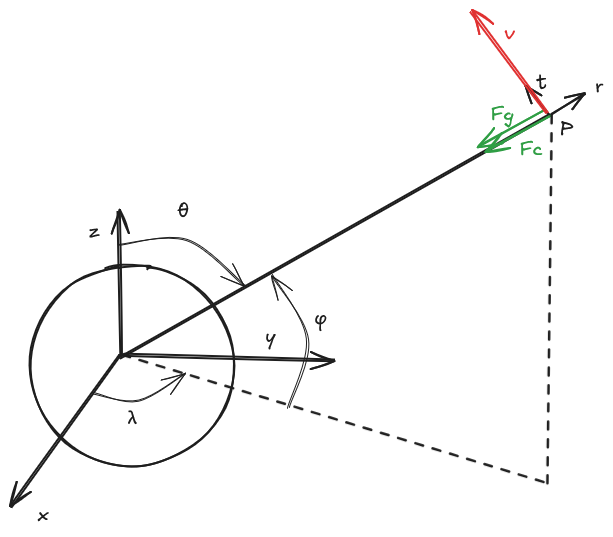
\includegraphics[scale=0.5]{satelite_schema.png}

The satellite position in a spherical referential $(\rho, \theta, \lambda)$ is : 

\begin{equation}
	\vec{OS} = 	\begin{bmatrix}
		l \\
		m\\
		n
	\end{bmatrix}_{R1} = \rho \cdot
		\begin{bmatrix}
		\sin(\theta) \cdot \cos(\lambda)\\
		\sin(\theta) \cdot \sin(\lambda)\\
		\cos(\theta)
	\end{bmatrix}_{R1}
\end{equation}
with
\begin{itemize}
	\item $\rho$ : radial distance from the center of the planet (origin) to the object, in meters.
	\item $\lambda$ : longitude, angle of rotation on the z axis
	\item $\phi$ : latitude of the satellite, elevation angle from the plane formed by x and y axes. (elevation angle, altitude angle)
	\item $\theta$ : polar angle between the polar axis(here the z axis) and the radial distance to the satellite. Or 	angle between the zenith and the latitude of the satellite at altitude $\phi$
	Complementary to $\phi$. (inclination angle, zenith angle, )
	$\theta = \frac{\pi}{2} - \phi$
	\item $\lambda$ : longitude, which is the azimuthal angle, which angle of rotation around the polar axis
\end{itemize}
 
 These angles are chosen to match the angles used for GPS location on Earth : latitude $\phi$ and longitude $\lambda$

TODO : express the velocity vector of the satellite 

\subsection{Stable orbit}
\subsubsection{Problem}
An artificial object (i.e a the satellite or a space craft)is orbiting around a space body at speed $v$ and at altitude $h_{sat}$. 
Calculate the force needed to maintain the object at that specific altitude

\subsubsection{Resolution}
Without any force applied on the artificial object, it will continue moving in the same direction as the speed vector. To maintain it constant altitude, i.e. forcing a circular trajectory around the planet, a centripetal force is applied toward the space body ($S$) center : 
\begin{equation}
	F_c = \frac{m_{sat} \cdot v_t^2}{\rho} = \frac{m_{sat} \cdot v_t^2}{S_{radius} + h_{sat}}
\end{equation}
\begin{equation}
	F_c = m_{sat} \cdot \omega^2 \cdot \rho= m \cdot (\frac{2 \pi}{T})^2 \cdot (S_{radius} + h_{sat})
\end{equation}

Todo : create table at the beginning describing each variables and its unit, 

$m_{sat}$ : mass of the orbiting object, in $kg$\\
$\rho$ : distance in $m$ from the center of the rotating object (planet, sun, moon) to the orbiting object\\
$v_t$ : tangential velocity of the orbiting object, in $m/s$\\
$S_{radii}$ : Space body radii, in $m$\\
$h_{sat}$ : distance from the surface of the space body to the satellite, in $m$\\
$\omega = \frac{2 \pi}{T}$ : angular speed of the space body, in $rad/s$\\
$T$ : orbital period, in $s$\\

In space, there are several ways to apply this force, like : 
\begin{itemize}
	\item gravity force, if the orbiting object is within the gravity field of the space body.
	\item thrusts applying force equal to $F_c$ at given time
\end{itemize}

CASE A : Gravity force\\
A.1. compute spped to stay at a given altitude\\
A.2. compute geostationary altitude, for different planets (check cases where the space body is gas and the satellite must orbit inside it)\\
CASE B : thrusters force : \\
compute fuel needed to maintain this (like for the ISS)

\subsubsection{Case A : Satellite within space body's gravity field}

\begin{eqnarray}
	F_c = m_{sat} \cdot g \\
	m_{sat} \cdot \frac{v_t^2}{\rho}  = m_{sat} \cdot \omega^2 \cdot \rho= m_{sat} \cdot g\\
	\frac{v_t^2}{\rho} = \omega^2 \cdot \rho = g =\frac{ G \cdot M_{S}}{\rho^2}\\
	v_t = \sqrt{\frac{ G \cdot M_{S}}{\rho}}\\
	\omega = \sqrt{\frac{ G \cdot M_{S}}{\rho^3}}\\
	\rho = \frac{ G \cdot M_{S}}{v_t^2}\\
	\rho = \sqrt[3]{\frac{ G \cdot M_{S}}{\omega^2}}
\end{eqnarray}

choose $v_t$ (or $\omega$) to stay at a specific orbit. Or if the orbiting object must have a specific speed, the altitude that it must reach is computed. Then, it is possible to check if the orbit at that altitude is free and can be used without colliding with other objects.
 
\subsubsection{Geostationary orbit}
Orbit where an object is moving at the same speed as the planet, and is always in the same position on the sky.
if it is satellite used for observation, it will look at exactly the same location on Earth. 
Some satellite follow this orbit, mainly for international communication. 
to maintain a the orbiting object, the object has the same angular speed as the space body $\omega=\omega_{S}$

\begin{eqnarray}
	\omega = \omega_{S}\\
	\rho_{go} = \sqrt[3]{\frac{ G \cdot M_{SB}}{\omega_{S}^2}}\\
	v_{go} = \omega_{S} \cdot r_{go}
\end{eqnarray}
Example for Earth : Period $T$ of 23h, 56min and 4s
\begin{eqnarray}
	T = 24*3600 + 56 * 60 + 4\\
	\omega = \omega_{Earth}= \frac{2 \cdot \pi}{T} = \frac{2 \cdot \pi}{23h 56min 4s}\\
	\rho_{go} = \sqrt[3]{\frac{ G \cdot M_{SB}}{\omega^2}}\\
	v_{go} = \omega_{S} \cdot r_{go}
\end{eqnarray}

As long as the orbiting object maintain this speed, it will stay at this orbit. However, friction with the high atmosphere might deviate the satellite from its path. some of them are equipped with thrusters to correct the trajectory when needed. 

Application example : 
- telecommunication satellites, placed around the planet to ensure that it is fully covered
- observation satellite : some satellites are placed to observe the same points of interest

\subsubsection{Case B : Orbit outside gravity field}
Altitude when gravity is very low
\begin{eqnarray}
	g = \frac{G \cdot M_S}{\rho ^2} <= 0.001\\
	\rho > \sqrt{\frac{G \cdot M_S}{g}}
\end{eqnarray}
Satellite is attracted by other space bodies, so thrusters and or boosters are needed to maintain the expected path. 

\begin{equation}
	\vec{v} = 	\begin{bmatrix}
		v_{\rho} \\
		v_{\theta}\\
		v_{\lambda}
	\end{bmatrix}_{R1}
\end{equation}
The components $v_{\theta}$ and $v_{\lambda}$ depends on the $v$ need to stay on orbit will maintain the satellite at orbit.
\begin{equation}
	v = \sqrt{v_{\theta}^2 + v_{\lambda}^2}
\end{equation}
The component $v_{\rho}$ must be compensated by activating thrusters and boosters to keep the altitude $\rho$ at the same value.


\subsubsection{les constantes}

\begin{itemize}
	\item G : 
	\item altitude de la position de départ
	\item k : coefficient caractéristique de la géométrie du solide
	\item $C_x$
	\item S : surface à l'air
	\item 
\end{itemize}


\begin{equation}
\vec{B_1 B_2}_{R_{1}}=
\begin{bmatrix}
v_1\cdot \cos(\beta_4) \\
0\\
v_1\cdot \sin(\beta_4)
\end{bmatrix}_{R1} \enspace
\vec{B_1 C_1}_{R_{1}}=
\begin{bmatrix}
c_1\cdot cos(\beta_1) \\
0\\
c_1\cdot sin(\beta_1)
\end{bmatrix}_{R1} \enspace
\vec{C_1 C}_{R_{1}}=
\begin{bmatrix}
c\cdot cos(\beta_1) \\
0\\
c\cdot sin(\beta_1)
\end{bmatrix}_{R1} \enspace
\end{equation}

\begin{equation}
\vec{C_1 C_2}=
\begin{bmatrix}
v_2\cdot cos(\gamma_1) \\
0\\
v_2 \cdot sin(\gamma_1)
\end{bmatrix}_{R1} \enspace
\vec{C C_2}_{R_{1}}=
\begin{bmatrix}
-c_2\\
0\\
0
\end{bmatrix}_{R2} \enspace
\vec{C_2 D}_{R_2}=
\begin{bmatrix}
-d\\
0\\
0
\end{bmatrix}_{R2} \enspace
\vec{D D_1}_{R_3}=
\begin{bmatrix}
- d_1\\
0\\
0
\end{bmatrix}_{R_3} \enspace
\end{equation}

\begin{equation}
\vec{D_1 D_2}_{R_3}=
\begin{bmatrix}
-d_2 \cdot cos(\delta_1)\\
0\\
d_2 \cdot sin(\delta_1)
\end{bmatrix}_{R_3} \enspace
\end{equation}

\begin{itemize}
	\item
	\item 
	\item 
\end{itemize}


\medbreak

\medbreak

\medbreak

\medbreak
L : longueur représentative de la fusée


\begin{eqnarray}
ggagsfaaf
\end{eqnarray}

\subsection{Formules utiles}
Reynolds number
\begin{equation}
	Re=\frac{\rho_{air} \cdot L \cdot v_{fusee}}{\mu}
\end{equation}


accélération terrestre
\begin{equation}
g= G \frac{m_{terre}}{(rayon_terre+altitude_{z_0}+z)^2}
\end{equation}

Force de pesanteur
\begin{equation}
Fg=m_fusee \cdot g
\end{equation}

frottement laminaire
\begin{equation}
Ffl=-k*\eta*v_{fusee}
\end{equation}

frottement turbulant
\begin{equation}
Fft=-\frac{1}{2} \cdot \rho_{air} \cdot C_x \cdot S \cdot v_{fusee}^2
\end{equation}

quantité de mouvement conservée

\begin{eqnarray}
	p_{fusee}=p_{gaz}\\
	P_{fusee}=m_{fusee}*v_{fusee}\\
	P_{gaz}=m_{gaz}*v_{gaz}\\
	dp/dt=somme F=m_{fusee}*a_{fusse}+ d m_{fusee}/dt+v_{fusee}\\
	dp/dt=m_gaz*a_gaz+d m_gaz/dt*v_{gaz}=F_{poussee}
\end{eqnarray}



equilibre des forces
\begin{eqnarray}
\sum F=F_{poussée}-F_g-F_{frottement}\\
a=\frac{\sum F}{m_{fusee}}
\end{eqnarray}
Les formules standards de la cinématique donnent vitesse et position. 
\begin{eqnarray}
v_{fusee}=a \cdot \Delta t\\
z=a \cdot \Delta t^2+v_{fusee} \cdot \Delta t+z_0
\end{eqnarray}



\subsection{Formules utiles}
nombre Reynolds
\begin{equation}
	Re=\frac{\rho_{air} \cdot L \cdot v_{fusee}}{\mu}
\end{equation}
accélération terrestre
\begin{equation}
	g= G \frac{m_{terre}}{(rayon_terre+altitude_{z_0}+z)^2}
\end{equation}

Force de pesanteur
\begin{equation}
	Fg=m_fusee \cdot g
\end{equation}

frottement laminaire
\begin{equation}
	Ffl=-k*\eta*v_{fusee}
\end{equation}

frottement turbulant
\begin{equation}
	Fft=-\frac{1}{2} \cdot \rho_{air} \cdot C_x \cdot S \cdot v_{fusee}^2
\end{equation}

quantité de mouvement conservée

\begin{eqnarray}
	p_{fusee}=p_{gaz}\\
	P_{fusee}=m_{fusee}*v_{fusee}\\
	P_{gaz}=m_{gaz}*v_{gaz}\\
	dp/dt=somme F=m_{fusee}*a_{fusse}+ d m_{fusee}/dt+v_{fusee}\\
	dp/dt=m_gaz*a_gaz+d m_gaz/dt*v_{gaz}=F_{poussee}
\end{eqnarray}
equilibre des forces
\begin{eqnarray}
	\sum F=F_{poussée}-F_g-F_{frottement}\\
	a=\frac{\sum F}{m_{fusee}}
\end{eqnarray}
Les formules standards de la cinématique donnent vitesse et position. 
\begin{eqnarray}
	v_{fusee}=a \cdot \Delta t\\
	z=a \cdot \Delta t^2+v_{fusee} \cdot \Delta t+z_0
\end{eqnarray}



\subsection{Procédure de calcul}

itérer à chaque pas de temps

calculer Re
selon valeur Re, le frottement est laminaire ou turbulant. limite environ vers 3000

force gravité
les frottements
équilibre des forces
accélération
pas de temps
vitesse 
positition

\subsection{Calcul plus poussé}
masse variable
quantité de mouvement et poussée des gaz. perte de masse à cause des gaz

g change selon l'altitude

les propriétés de l'air change, $\rho$, $\mu$, $\eta$, ...

$L$ de la fusée si elle perd des étages

calcul précis du $C_x$ : cf TAero, ou cours mécanique fluide incompressible EPFL
\subsection{Conclusion}

\subsection{Other cases}
1. establish the equation of the general movement of a satellite (the same as on Earth)

Acceleration
\begin{equation}
	\vec{a}=\frac{\sum \vec{F}}{m_{sat}}
\end{equation}
Force equilibrium in a spherical referential (check if this is correct. maybe another force must be added. Centripetal force is only tangential)
\begin{equation}
	\sum \vec{F}=\vec{F_{c}}-\vec{F_g} = \vec{F_R} = 
	\begin{bmatrix}
		F_c\cdot cos(\alpha) \\
		F_c\cdot sin(\alpha)\\
		0
	\end{bmatrix}_{R1} + 
	\begin{bmatrix}
		- F_g \\
		0\\
		0
	\end{bmatrix}_{R1} = m_{sat} \cdot	\begin{bmatrix}
		a_r \\
		a_t\\
		a_z
	\end{bmatrix}_{R1}
\end{equation}

\begin{eqnarray}
	F_c\cdot cos(\alpha) = m_{sat} \cdot g \\
	m_{sat} \cdot \frac{v_t^2}{r} \cdot cos(\alpha) = m_{sat} \cdot \omega^2 * r \cdot cos(\alpha)= m_{sat} \cdot g\\
	\frac{v_t^2}{r} \cdot cos(\alpha) = \omega^2 \cdot r \cdot cos(\alpha) = g =\frac{ G \cdot m_{Earth}}{r^2}\\
	v_t = \sqrt{\frac{ G \cdot m_{Earth}}{r\cdot cos(\alpha)}}\\
	\omega = \sqrt{\frac{ G \cdot m_{Earth}}{r^3\cdot cos(\alpha)}}\\
\end{eqnarray}

2. Drag and lift forces depend if there is an atmosphere or not at that altitude
-> compute air density depending on altitude. it will become 0 in space
3. simulate different cases with different propulsion, ....

4. test case : propulsion force that must be applied to maintain orbit over the planet (Earth)

5. the same case but using gravity force

6. so the same calculations for all planets and moon in the solar system

7. ignore sun heat and radiation, do the same with the sun 


8. other case : how close a satellite be from the sun ? can a satellite orbit around it ? will it susstain the heat, the radiation form the sun ?

\section{Putting a rocket in orbit}

\subsection{Introduction}

Etudier la cinématique du lancement et de la mise en orbite d'une fusée
\medbreak
la mise en orbite sera faite en prenant en compte les aspects dynamiques


\newpage
\subsection{Schémas}
schéma représentatif de la situation

schéma de l'atmosphère, avec formules de températures et pression selon altitude

\subsection{Etude cinématique}


\subsubsection{les constantes}

\begin{itemize}
	\item G : 
	\item altitude de la position de départ
	\item k : coefficient caractéristique de la géométrie du solide
	\item $C_x$
	\item S : surface à l'air
	\item 
\end{itemize}


\begin{equation}
	\vec{B_1 B_2}_{R_{1}}=
	\begin{bmatrix}
		v_1\cdot cos(\beta_4) \\
		0\\
		v_1\cdot sin(\beta_4)
	\end{bmatrix}_{R1} \enspace
	\vec{B_1 C_1}_{R_{1}}=
	\begin{bmatrix}
		c_1\cdot cos(\beta_1) \\
		0\\
		c_1\cdot sin(\beta_1)
	\end{bmatrix}_{R1} \enspace
	\vec{C_1 C}_{R_{1}}=
	\begin{bmatrix}
		c\cdot cos(\beta_1) \\
		0\\
		c\cdot sin(\beta_1)
	\end{bmatrix}_{R1} \enspace
\end{equation}

\begin{equation}
	\vec{C_1 C_2}=
	\begin{bmatrix}
		v_2\cdot cos(\gamma_1) \\
		0\\
		v_2 \cdot sin(\gamma_1)
	\end{bmatrix}_{R1} \enspace
	\vec{C C_2}_{R_{1}}=
	\begin{bmatrix}
		-c_2\\
		0\\
		0
	\end{bmatrix}_{R2} \enspace
	\vec{C_2 D}_{R_2}=
	\begin{bmatrix}
		-d\\
		0\\
		0
	\end{bmatrix}_{R2} \enspace
	\vec{D D_1}_{R_3}=
	\begin{bmatrix}
		- d_1\\
		0\\
		0
	\end{bmatrix}_{R_3} \enspace
\end{equation}

\begin{equation}
	\vec{D_1 D_2}_{R_3}=
	\begin{bmatrix}
		-d_2 \cdot cos(\delta_1)\\
		0\\
		d_2 \cdot sin(\delta_1)
	\end{bmatrix}_{R_3} \enspace
\end{equation}


\section{Kinematics}
\subsection{Introduction}

The objective of this report is to compute the trajectory of a projectile following the ballistic mechanics. 

% 
\includegraphics[scale=.2]{oxford-2021-01.jpg}

\subsection{Examples}

Hitting moving target with unguided rockets


\subsection{Initial conditions}

projectile initial positions : 
\begin{eqnarray}
	px = px_0 + pv * cos(p_{alpha}) * \Delta t\\
	py = py_0 + pv * sin(p_{alpha}) * \Delta t
\end{eqnarray}

Target positions : 
\begin{eqnarray}
	Tx = Tx_0 + Tv * cos(T_{alpha}) * \Delta t\\
	Ty = Ty_0 + Tv * sin(T_{alpha}) * \Delta t
\end{eqnarray}

The target is hit when :
\begin{eqnarray}
	Tx = px\\
	Tx_0 + Tv * cos(T_{alpha}) * \Delta t = px_0 + pv * cos(p_{alpha}) * \Delta t\\
	(Tx_0 - px_0) + [Tv * cos(T_{alpha})-pv * cos(p_{alpha}) ] * \Delta t =  0
\end{eqnarray}

\begin{eqnarray}
	Ty = py \\
	Ty_0 + Tv * sin(T_{alpha}) * \Delta t = py_0 + pv * sin(p_{alpha}) * \Delta t\\
	(Ty_0 -py_0) + [Tv * sin(T_{alpha}) - pv * sin(p_{alpha})] * \Delta t = 0
\end{eqnarray}


\begin{eqnarray}
	(Tx_0 - px_0) + [Tv * cos(T_{alpha})-pv * cos(p_{alpha}) ] * \Delta t =  0 \\
	(Ty_0 -py_0) + [Tv * sin(T_{alpha}) - pv * sin(p_{alpha})] * \Delta t = 0
\end{eqnarray}

In this problem, we have 2 unknown variables : $\Delta t$ and $p_{alpha}$.


Launching angle : $alpha$

Propulsion force : $F_p$

Gravity force : $F_g$

If the projectile is launched from a canon, 
friction with cannon : $F_{friction}$
We will discuss this case at the end of the report. 

\subsection{Reynolds Number}
The Reynolds number is an non-dimensional number, and used to define if the fluid flow is laminar or turbulent. 

\begin{equation}
	Re = \frac{\rho \cdot u \cdot L}{\mu}
\end{equation}
$\rho$ : density of the fluid\\
$u$ : flow speed\\
$L$ : characteristic linear dimension\\
$\mu$ : dynamic viscosity of the fluid\\

The characteristic linear dimension $L$ depends on the shape of the object of study. Here some example : 
\begin{itemize}
	\item Plane wing : length of the wing
	\item Hydraulic pipe : diameter of the pipe
	\item Complex shape : the biggest dimension
\end{itemize}
Depending of the result, the flow can have 3 regimes

\begin{itemize}
	\item If $Re$ <~ 2040, the flow is still considered laminar 
	\item If $Re$ >~ 2100, the flow is turbulent
	\item If 1800 <~ $Re$ <~ 2100, the flow is in the transition/intermediary range, which is a mix of laminar and turbulent \footnote{\url{https://en.wikipedia.org/wiki/Laminar_flow}}
\end{itemize}

For each regime, the drag force is different. 
For turbulent and laminar regimes, the formula is as follows:
\begin{equation}
	F_d^{turbulent} = \frac{1}{2} \cdot \rho \cdot C_D \cdot S \cdot u^2
\end{equation}

\begin{equation}
	F_d^{laminar} = C_F \cdot \rho \cdot  D^2 \cdot u^2\\
\end{equation}
$S$: cross frontal section\\
$C_D$ : turbulent drag coefficient\\
$C_F$ : laminar drag coefficient\\

The intermediary regime is a mix from the 2 base regimes. In this situation, an approximation can be evaluated by computed the percent $Re$ compared to 1800 and 2100. 
\begin{equation}
	F_d^{transition} = (1- \frac{Re - 1800}{2100-1800}) \cdot F_d^{laminar} + \frac{Re - 1800}{2100-1800} \cdot F_d^{turbulent}
\end{equation}

\subsection{Cannon cinematic}
In this case, we need to consider what happens to the projectile inside the barrel, from the moment the projectile starts moving until it exits the barrel. 

The projectile is launched by the mean of an explosive charge placed in the breach. 
When the shooter presses on the fire button, this charge is set off. 

The energy of the charge is used as propulsion energy for the projectile. A small portion of the energy is used to spin the projectile, which will stabilize the trajectory during the flight. 

\begin{eqnarray}
	E_{charge} = E_{kin}^{translation} + E_{kin}^{rotation} \\
	E_{charge} = \frac{1}{2} \cdot m_{projectile} \cdot v^2 + \frac{1}{2} \cdot I \cdot \omega ^ 2
\end{eqnarray}

To push the projectile, the energy of the charge will generate a pressure. Using the definition of the pressure and energy as functions of force, it is possible to define the pressure as function of energy. 

\begin{eqnarray}
	p = F/A \\
	E = F \cdot d \\
	p = \frac{F}{A \cdot d} = \frac{E}{V}
\end{eqnarray}

In our example, the energy used to move the projectile is the kinetic energy of translation $E_{kin}^{translation}$, $F$ is the propulsion force $F_p$, and $V$ is the initial volume of the exploded charge (gas).
\begin{eqnarray}
	p_{charge} = \frac{F_p}{A \cdot d} = \frac{E_{kin}^{translation}}{V_{charge}}
\end{eqnarray}

\subsubsection{Charge/explosion volume}
\begin{eqnarray}
	V_{charge}^{inital} = A_{ projectile} \cdot h_{projectile} =  \frac{D_{projectile}^2}{4} \cdot h_{projectile}
\end{eqnarray}
After the charge is set off, this volume will change

\begin{eqnarray}
	V(t) = V_{charge}^{inital} + Position_{projectile}(t) \cdot A_{projectile}
\end{eqnarray}

\subsubsection{Propulsion pressure}

In reality, we need to consider the atmospheric pressure. 
\begin{eqnarray}
	P_{charge} - p_{atm} = \frac{F_p}{A \cdot d} = \frac{E_{kin}^{translation}}{V_{charge}}
\end{eqnarray}


After the charge is set off, the projectile starts moving by the action of $P_{charge}$ on its section $A_{projectile}$, which induces the propulsion force $F_p$. 
\begin{equation}
	F_p = P_{charge} \cdot A_{projectile} =  P_{charge} \cdot \pi \cdot \frac{D_{projectile}^2}{4}
\end{equation}
As the projectile is moving away from the breech, $ V_{charge}$ will increase and thus the pressure is reduced. Consequently, the pressure will keep pushing the projectile, but with lower propulsion force. This ends with one of these situations happens:  
\begin{itemize}
	\item The projectile is out the barrel
	\item $P_{charge}$ is equal to $p_{atm}$
\end{itemize}

\subsubsection{Projectile spinning}
To stabilize its trajectory during its flight and increase the range, the projectile should spin with a specified angular speed. This is achieved by the thread inside the barrel. The mathematics formula is as follows :  
\begin{eqnarray}
	E_{kin}^{rotation} = \frac{1}{2} \cdot I \cdot \omega ^ 2
\end{eqnarray}
The spinning will produce an angular momentum $L$:
\begin{eqnarray}
	L = m \cdot v \cdot r
\end{eqnarray}
where, 
$m$ : is the projectile mass
$v$ : projectile velocity
$r$ : projectile radium

The rotational kinetic energy is the highest the moment the projectile exits the barrel. During the flight and due to the friction with air, the spinning is reduced.
this value should be optimized because
- to produce this spinning, the projectile has friction with the internal diameter of the barrel. The threads will initiate the projectile rotation. 

the more the friction, the higher is the spinning, but it will also reduce the kinetic energy, -> lower velocity

if the friction is not enough, rotational energy is low, the trajectory is not stabilized enough and the accuracy of the shot is low. 

For this, test with different 
- spinning thread shape and number
- barrel length
- explosive charge. 

The angular momentum must be optimized.

To make sure it is optimized, the shell is placed on a test bench, submitted to a wind flow. This simulated the shell during the flight. in the same time, the projectile is spinning. 
the wind flow is reduced to simulate the air that slows the energy of the projectile. during the simulation, we measure the angular momentum and its resulting force to find if it will stays on the computed trajectory. 
the angular speed is controlled at the beginning of the simulation, when the shell exits the barrel. 

\newpage

table

\begin{table}[ht]
	\caption{Holes and threaded holes} % title of Table
	\centering % used for centering table
	\begin{tabular}{c c c} % centered columns (4 columns)
		\hline\hline %inserts double horizontal lines
		Screw & Threaded hole diameter & Bore Hole (clearance) \\ [0.5ex] % inserts table
		%heading
		\hline % inserts single horizontal line
		M3 & 2.8 & 3.2 \\ % inserting body of the table
		4 & 35 & 144 \\
		5 & 45 & 300 \\ [1ex] % [1ex] adds vertical space
		\hline %inserts single line
	\end{tabular}\label{table:nonlin} % is used to refer this table in the text
\end{table}

Clearance
To fix two part together, a clearance is needed.
When two parts must be assembled together, a clearance of 0.1mm is enough. Then use the glue to fix the assembly. 



\begin{table}[ht]
	\caption{Nonlinear Model Results} % title of Table
	\centering % used for centering table
	\begin{tabular}{c c c c} % centered columns (4 columns)
		\hline\hline %inserts double horizontal lines
		Case & Method\#1 & Method\#2 & Method\#3 \\ [0.5ex] % inserts table
		%heading
		\hline % inserts single horizontal line
		1 & 50 & 837 & 970 \\ % inserting body of the table
		2 & 47 & 877 & 230 \\
		3 & 31 & 25 & 415 \\
		4 & 35 & 144 & 2356 \\
		5 & 45 & 300 & 556 \\ [1ex] % [1ex] adds vertical space
		\hline %inserts single line
	\end{tabular}\label{table:nonlin} % is used to refer this table in the text
\end{table}



\begin{equation}
	Length_{lattitude}(\phi) = 111132.92-559.82 \cdot cos(2 \cdot \phi)+1.175*cos(4 \cdot \phi)-0.0023 \cdot cos(6 \cdot \phi)= ... [m/degree]
\end{equation}
1 degree longitude at latitude phi
\begin{equation}
	Length_{longitude}(\phi) =
	111412.84-93.5 \cdot cos(3 \cdot \phi)+ 0.118 \cdot cos(5 \cdot \phi)= ... [m/degree]
\end{equation}

\newpage
\subsection{Collisions}
https://www.youtube.com/watch?v=M2xnGcaaAi4

\subsubsection{Elastic collision}
Momentum is conserved
\begin{eqnarray}
	\sum_{i} \vec{p_i} = \vec{P}\\
	m_1 \cdot \vec{v_{1i}} + m_2 \cdot \vec{v_{2i}} = m_1 \cdot \vec{v_{1f}} + m_2 \cdot \vec{v_{2f}}
\end{eqnarray}
Energy is conserved 
\begin{equation}
	E_{kin}^i = E_{kin}^f = \frac{1}{2} \cdot m \cdot v_1^2 =  \frac{1}{2} \cdot m \cdot v_2^2
\end{equation}
\subsubsubsection{Pool balls}
\subsubsubsection{Ricochet}
An object is bouncing off a solid surface.

The object collides on the surface with an angle $\theta$ to the normal vector and will bounce off with the same angle. 

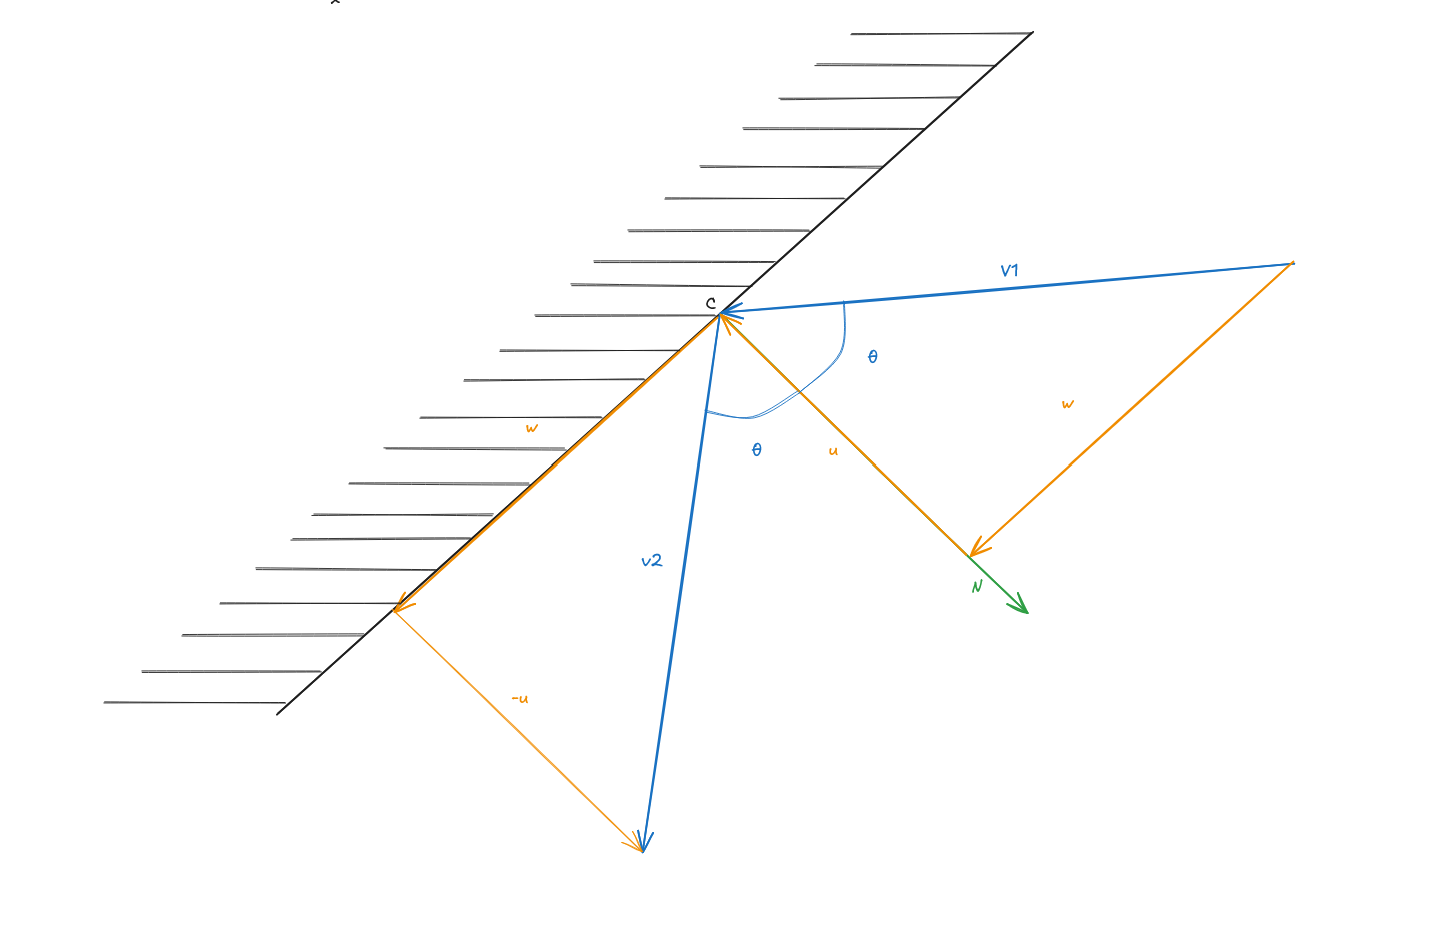
\includegraphics[scale=0.8]{ricochet.png}

We consider a perfect elastic collision. 
- bodies in collision stay separate after
- No Energy losses : Energy is conserved
\begin{equation}
	E_{kin}^i = E_{kin}^f = \frac{1}{2} \cdot m \cdot v_1^2 =  \frac{1}{2} \cdot m \cdot v_2^2
\end{equation}

Velocity vector can be projected on the surface and its normal : 
\begin{eqnarray}
	\vec{v_1} = \vec{u} + \vec{w}
\end{eqnarray}
$\vec{u}$ is the projection of $\vec{v_1}$ on the surface normal $\vec{n}$
\begin{eqnarray}
	\vec{u} = \frac{\vec{v_1} x \vec{n}}{\vec{n} x \vec{n}} \vec{n}\\
	\vec{w} = \vec{v_1} - \vec{u}
\end{eqnarray}
where $x$ is the scalar product. 
\begin{equation}
	\vec{v_2} = \vec{w} - \vec{u}
\end{equation}
\subsubsection{Near elastic collision}
bodies stay separate, energy is lost to sound and heat
\begin{equation}
	E_{kin}^i = E_{kin}^f + E_{heat} + E_{sound}
\end{equation}
\subsubsection{Plastic collision}
\subsubsection{Perfect Inelastic collision}
Energy is also lost in deformation, like 
2 cars in collision and stay together after 

Momentum
\begin{equation}
	m_1 \cdot v_1 + m_2 \cdot v_2 = (m_1 + m_2) \cdot v_f
\end{equation}
\begin{equation}
	E_{kin}^i = E_{kin}^f + E_{heat} + E_{sound} + E_{deformation}
\end{equation}
\newpage
\subsection{Schéma cinématique}


\subsection{Vecteurs positions}
origine : centre de rotation verticale se trouvant sous les pâles principales.
\medbreak
position  des pâles principales ($pp$) : vecteur verticale
\medbreak
position de l'hélice arrière : 
vecteur allant de l'origine vers l'hélice ($h$) arrière. 


\newpage
\subsection{Angular momentum}

\subsubsection{Formula}
\begin{equation}
	\vec{L}=\vec{OA} \otimes \vec{P}=\vec{r} \otimes \vec{P}=\vec{r} \otimes m \cdot \vec{v}=\vec{I} \otimes \vec{\omega}
\end{equation}
$\vec{L}$ : Angular Momentum [$kg \cdot \frac{m^2}{s}$]\\
$\vec{OA}$ and $r$: position of the mass [$m$] according to a referance\\
$\vec{P}$ : linear momentum [$kg\cdot \frac{m}{s}$]\footnote{$\vec{L}$ is perpendicular to both $\vec{P}$ and $\vec{r}$}\\
$\vec{v}$ : velocity [$\frac{m}{s}$]
$I$ : moment of inertia [$m^2 \cdot kg \cdot$]\\
$\omega$ : angular speed [$\frac{rad}{s}$]

Torque : 
\begin{equation}
	M = \frac{d\vec{L}}{dt}=\frac{d(\vec{I} \otimes \vec{\omega})}{dt}
\end{equation}
\medbreak
if we consider a particule of mass $m$, $\vec{r}$ is the position of the center of mass.
If it is a solid object, $L$ is first computed according to the axis of rotation of the object : 
\begin{equation}
	\vec{L}_{ar}=\vec{I}_{ar} \otimes \vec{\omega}_{ar}
\end{equation}
To compute the angular moment according to an other axis of rotation (new referance), we use the Huygens-Steiner theorem (or the Parallel axis theorem) : 
\begin{equation}
	\vec{L}_{0}=\vec{I}_{0} \otimes \vec{\omega}_{cm}\\
\end{equation}
\begin{equation}
	\vec{I}_{0} = \vec{I}_{ar} + m\cdot d^2
\end{equation}
with $d$ the distance between the axis of rotation of the object and the new referance. 
\subsubsection{Condition of stability}

Main rotor(s):
\begin{equation}
	\vec{L}_{mr}=\vec{r}_{mr} \otimes m_{mr} \cdot \vec{v_{mr}}=\vec{I_{mr}} \otimes \vec{\omega_{mr}}
\end{equation}


Rear rotor : 
\begin{equation}
	\vec{L}_{rr}=\vec{r}_{rr} \otimes m_{rr} \cdot \vec{v_{rr}}=\vec{I_rr} \otimes \vec{\omega_{rr}}
\end{equation}

assurer la stabilité lors du vol: les moments cinétiques doivent s'annuler. (poser la formule et résoudre)
\begin{equation}
	\vec{L_{mr}}=\vec{L_{rr}}
\end{equation}

or

The generated torque is compensated : 
\begin{equation}
	\sum \vec{M_{mr}}=\sum \vec{M_{rr}}
\end{equation}

find a relation between $\omega_{mr}$ and $\omega_{rr}$ -> determine the transmission ratio

\subsubsection{Pivots à droite et à gauche}
pour tourner à gauche ou doite, on ne doit plus satisfaire la condition de stabilité. le pilote utiliser le pédalier pour accélérer/ralentir l'hélice arrière. ainsi les moments cinétiques ne sont plus égaux.
\medbreak
calculer l'effet de rotation sur l'hélicoptère si l'hélice est accélérée/ralentie de 10,20,30,.. $\%$. mettre un tableau. calculer la vitesse de rotation dans ces cas-là. 


\begin{equation}
	\begin{bmatrix}
		0 \\
		0\\
		l_1
	\end{bmatrix}_{R_{1}} \enspace
	\vec{AB}_{R_{2}}=
	\begin{bmatrix}
		0 \\
		l_2\\
		0
	\end{bmatrix}_{R_{2}} \enspace
	\vec{BC}_{R_{3}}=
	\begin{bmatrix}
		l_3 \\
		0\\
		0
	\end{bmatrix}_{R_{3}} \enspace
	\vec{CD}_{R_{4}}=
	\begin{bmatrix}
		0 \\
		0\\
		-l_4
	\end{bmatrix}_{R_{4}} \enspace
\end{equation}

\begin{itemize}
	\item
	\item 
	\item 
\end{itemize}


\medbreak

\medbreak

\medbreak

\medbreak




\begin{equation}
	\begin{split}
		\vec{OE}_R=\vec{OA}_R+\vec{AB}_R+\vec{B B_1}_R+\vec{B_1 C_1}_R+\vec{C_1 C}_R\\+\vec{C C_2}_R+\vec{C_2 D}_R+\vec{D D_1}_R+\vec{D_1 E}_R
	\end{split}
\end{equation}

\begin{equation}
	\begin{split}
		\vec{OF}_R=\vec{OA}_R+\vec{AB}_R+\vec{B B_1}_R+\vec{B_1 C_1}_R+\vec{C_1 C}_R\\+\vec{C C_2}_R+\vec{C_2 D}_R+\vec{D D_1}_R+\vec{D_1 E}_R+\vec{E F}_R
	\end{split}
\end{equation}

\begin{equation}
	\begin{split}
		\vec{OG}_R=\vec{OA}_R+\vec{AB}_R+\vec{B B_1}_R+\vec{B_1 C_1}_R+\vec{C_1 C}_R+\vec{C C_2}_R\\+\vec{C_2 D}_R+\vec{D D_1}_R+\vec{D_1 E}_R+\vec{E F}_R+\vec{F F_3}_R+\vec{F_3 G}_R
	\end{split}
\end{equation}

\begin{equation}
	\begin{split}
		\vec{OH}_R=\vec{OA}_R+\vec{AB}_R+\vec{B B_1}_R+\vec{B_1 C_1}_R+\vec{C_1 C}_R+\vec{C C_2}_R+\vec{C_2 D}_R\\+\vec{D D_1}_R+\vec{D_1 E}_R+\vec{E F}_R+\vec{F F_3}_R+\vec{F_3 G}_R+\vec{G H}_R
	\end{split}
\end{equation}


\subsection{Conclusion}



\end{document}